\chapter{Tema 2: Grupos. Definición, generalidades y ejemplos}

\begin{definicion}
    Sea $G$ un conjunto, una \textbf{operación binaria} en $G$ es una aplicación
    \begin{align*}
        \ast : G\times G &\to G\\
        (a,b) & \mapsto a\ast b = a \cdot b = ab
    \end{align*} 
\end{definicion}

\begin{ejemplo}\
    \begin{enumerate}
        \item Suma y producto en $\bb{N}, \bb{Z}, \bb{R}$
        \item Dado $X$ un conjunto, $\cc{P}(X)$, $\cup, \cap $ son operaciones binarias.
    \end{enumerate}
\end{ejemplo}

\begin{definicion}
    Un \textbf{monoide} es un conjunto no vacío junto con una operación binaria verificando:
    \begin{enumerate}
        \item[i)] La propiedad asociativa: $(x\ast y) \ast z = x \ast (y \ast z)$
        \item[ii)] Existencia de elemento neutro: $\exists e \in G$ tal que $e\ast x = x$ \ \ $\forall x \in G$
    \end{enumerate}
\end{definicion}

\begin{lema}
    En un monoide el neutro es único.
\end{lema}

\begin{ejemplo}\
    \begin{enumerate}
        \item $(\bb{N},+,0)$, $(\bb{N},\times,1)$
        \item $(\cc{P}(X), \cap, X)$, $(\cc{P}(X), \cup, \emptyset)$
    \end{enumerate}
\end{ejemplo}

\begin{definicion}
    Un \textbf{grupo} es un conjunto no vacío junto con una operación binaria verificando:
    \begin{enumerate}
        \item[i)] La propiedad asociativa: $(x\ast y) \ast z = x \ast (y \ast z)$
        \item[ii)] Existencia de elemento neutro: $\exists e \in G$ tal que $e\ast x = x$ \ \ $\forall x \in G$
        \item[iii)] Existencia de elemento simétrico: $\forall x \in G$\ \ $\exists x'\in G$ tal que $x\ast x' = e$
    \end{enumerate}
    y si además se cumple que 
    \begin{enumerate}
        \item[iv)] Propiedad conmutativa: $x\ast y = y \ast x$\ \ $\forall x,y\in G$ 
    \end{enumerate}
    Entonces $G$ es un \textbf{grupo abeliano}.
\end{definicion}

\begin{observacion}\
    \begin{enumerate}
        \item $(G,\ast,e) \leadsto G$
        \item Notación multiplicativa: 
        \begin{itemize}
            \item $x\ast y = xy$
            \item Neutro $\leadsto 1$
            \item simétrico $\leadsto$ inverso $x^{-1}$
        \end{itemize}
        \item Notación aditiva: 
        \begin{itemize}
            \item $x+ y$
            \item Neutro $\leadsto 0$
            \item simétrico $\leadsto$ opuesto $-x$
        \end{itemize}
    \end{enumerate}
\end{observacion}

\begin{ejemplo}\
    \begin{enumerate}
        \item $\bb{Z}, \bb{Q}, \bb{R}, \bb{C}$ con la suma son grupos abelianos.
        \item $\bb{Q}^*, \bb{R}^*, \bb{C}^*$ con el producto son grupos abelianos.
        \item $\{1,-1,i,-i\}\subset \bb{C}$ con el producto es un grupo abeliano.
        \item $(\cc{M}_2(\bb{R}), +)$ es un grupo abeliano
        \item $GL_2(\bb{R})$ el grupo lineal de orden $2$ con el producto es un grupo (pero no abeliano, ya que el producto de matrices no es conmutativo).
        \begin{align*}
            GL_2(\bb{R}) = \{A\in \cc{M}_2(\bb{R}) \text{ tal que }\det(A)\neq 0\}
        \end{align*}
        \item $\bb{Z}_n$ con la suma es un grupo abeliano.
        \item $U(\bb{Z}_n)=\{\overline{a}\in \bb{Z}_n \text{ tal que } m.c.d(a,n)=1\}$ con la multiplicación (multiplicación de clases) es un grupo abeliano. Por ejemplo:        
        \begin{align*}
            U(\bb{Z}_4) = \{1,3\} \hspace*{1cm} 1\cdot 1 = 1 ,\ 3\cdot 3 = 1
        \end{align*}
        \item $n\geq 1$, $\mu_n=\{$raíces complejas de $x^n-1\} = \{\xi_k = \cos \frac{2k \pi}{n} + i \sen \frac{2k \pi}{n},\ k=0,\dots,n-1\}=\{1, \xi, \xi^2, \dots, \xi^{n-1}\text{ tal que } \xi=\cos \frac{2 \pi}{n} + i \sen \frac{2 \pi}{n}\}$ es un grupo abeliano con el producto.
        \item $SL_2(\bb{K})=\{$matrices con $\det=1\}$ con $\bb{K}$ un cuerpo con el producto de matrices es un grupo.
        \item $G$ y $H$ grupos, $G\times H$ es un grupo con $(x,y)\ast(x',y')=(xx',yy')$ y se llama \textbf{producto directo} de $G$ y $H$.
        \item Sea $X$ un conjunto no vacío. Consideramos 
        \begin{align*}
            S(X)=\{f:X\to X \text{ biyectivas}\}
        \end{align*}
        el conjunto de las permutaciones de $X$. Con la composición es un grupo. Llamaremos a este grupo $S_n$ donde $n$ será el número de elementos de $X$, $X=\{1,2,\dots,n\}$.
        \item Sean $G$ un grupo, $X$ un conjunto. Consideramos
        \begin{align*}
            Apl(X,G) = G^X = \{f:X \to G \text{ aplicaciones}\}
        \end{align*}
        podemos definir $(f\ast g)(x) = f(x)g(x)$. Si $f\in G^X$, tendremos que $f'(x)=(f(x))'$.\\

        Si $X=\emptyset$, entonces $G^X=\{\emptyset\}$ y si $X=\{1,2\}$, entonces $G^X$ es isomorfo a $G\times G$.
    \end{enumerate}
\end{ejemplo}

\begin{lema}
    Sea $G$ un grupo, entonces
    \begin{enumerate}
        \item[i)] $xx^{-1} = e$\ \ $\forall x \in G$.
        \item[ii)] $x e = x$\ \ $\forall x \in G$.
    \end{enumerate}
    \begin{proof}\
        \begin{enumerate}
            \item[i)] $x^{-1}(x x^{-1}) = (x^{-1} x)x^{-1} = e x^{-1} = x^{-1}$
            \item[ii)] $xe = x(x^{-1}x) = (x x^{-1})x = ex = x$ 
        \end{enumerate}
    \end{proof}
\end{lema}

\begin{lema}
    En un grupo $G$, el neutro del grupo y el simétrico de cada elemento son únicos.
    %TODO: demostración (suponiendo que hay 2)
\end{lema}

\begin{lema}
    (Propiedad cancelativa). \
    \begin{align*}
        \forall x,y,z\in G \left\{
        \begin{array}{l}
            xy = xz \Rightarrow y=z\\
            xy = zy \Rightarrow x=z
        \end{array}
        \right.
    \end{align*}
    \begin{proof}
        Para el primer caso tenemos $y=ey=(x^{-1}x)y = x^{-1}(xy)=x^{-1}(xz)=(x^{-1}x)z = ez = z$. El segundo caso es análogo %TODO
    \end{proof}
\end{lema}

\begin{lema}
    Sea $G$ un grupo, entonces
    \begin{enumerate}
        \item[i)] $e^{-1} = e$
        \item[ii)] $(x^{-1})^{-1}=x$\ \ $\forall x \in G$.
        \item[iii)] $(xy)^{-1} = y^{-1}x^{-1}$\ \ $\forall x,y\in G$.
    \end{enumerate}
    \begin{proof}\
        \begin{enumerate}
            \item[i)] $ee=e$
            \item[ii)] $xx^{-1=e} \Rightarrow (x^{-1})^{-1} = x$.
            \item[iii)] $(y^{-1}x^{-1})(xy) = y^{-1}x^{-1}xy = y^{-1} e y = y^{-1}y = e$
        \end{enumerate}
    \end{proof}
\end{lema}

\begin{lema}
    Sea $G$ un conjunto no vacío con una operación binaria asociativa. Entonces son equivalentes:
    \begin{enumerate}
        \item[i)] $G$ es un grupo.
        \item[ii)] Para cada par de elementos $a,b\in G$, las ecuaciones $aX=b$, $Xa=b$ tienen solución en $G$, es decir, que $\exists c,d\in G$ de forma que $ac=b$ y $da=b$, en cuyo caso $c$ y $d$ son las soluciones de la ecuación. 
    \end{enumerate}
    \begin{proof}\
        \begin{itemize}
            \item[i) $\Rightarrow$ ii) )] $aX=b \Rightarrow c=a^{-1}b$ y $Xa=b\Rightarrow d=ba^{-1}$.
            \item[ii) $\Rightarrow$ i) )] Sabemos que $aX=b$ tiene solución y la notamos por $e_a$. Consideramos también $\forall b\in G$, $Xa=b$ y tomamos $x$ tal que $xa=b$. Entonces $be_a = xae_a = xa = b \Rightarrow e_a \leadsto e$ es un neutro por la derecha. Por tanto tenemos que $aX=e \leadsto \exists a^{-1} \Rightarrow G$ es un grupo. 
        \end{itemize}
    \end{proof}
\end{lema} 

\begin{lema}
    (Ley asociativa general)\\
    Sea $G$ un grupo, $\forall x \in G$, $\forall m,n>0$ con $n>m>0$, entonces se tiene
    \begin{align*}
        \left(\prod\limits_{i=1}^m x_i\right)\left(\prod\limits_{i=m+1}^n x_i\right) = \prod\limits_{i=1}^n x_i
    \end{align*}

    % La demostración se hace por inducción
\end{lema}

\begin{definicion}
    Potencia
    \begin{align*}
        x^n = \left\{
        \begin{array}{ll}
            x^n & n>0\\
            e & n=0\\
            (x^{-1})^{-n} & n<0
        \end{array}
        \right.\hspace{2cm} x^{n+m}=x^n \cdot x^m
    \end{align*}
\end{definicion}

\begin{definicion}
    Sea $G$ un grupo, si $G$ tiene un número finito de elementos, entonces se llama \textbf{grupo finito} y a ese número de elementos se le llama orden del grupo y lo notaremos por $|G|$.
\end{definicion}

\begin{definicion}
    (Tabla de Cayley)\\
    En un grupo finito $G=\{x_1=1, x_2, \dots, x_n\}$  se llama \textbf{tabla de Cayley} (o tabla de multiplicar) a la matriz $n\times n$ cuya entrada $(i,j)$ es $x_ix_j$.
\end{definicion}

\begin{ejemplo}\
    \begin{itemize}
        \item $G=\{0,1\}$

        \begin{tabular}{c|c|c|}
            $\ast_1$ & 0 & 1\\
            \hline
            0 & 0 & 1\\
            \hline
            1 & 1 & 0\\
            \hline
        \end{tabular}

        \ \\

        \begin{tabular}{c|c|c|}
            $\ast_2$ & 0 & 1\\
            \hline
            0 & 1 & 0\\
            \hline
            1 & 0 & 1\\
            \hline
        \end{tabular}

        \item $G=\{0,1,2\}$

        \begin{tabular}{c|c|c|c|}
            $+$ & 0 & 1 & 2\\
            \hline
            0 & 0 & 1 & 2\\
            \hline
            1 & 1 & 2 & 0\\
            \hline
            2 & 2 & 0 & 1\\
            \hline
        \end{tabular}

        \item $G=\{0,1,2,3\}$

        \begin{tabular}{c|c|c|c|c|}
             & 0 & 1 & 2 & 3\\
            \hline
            0 & 0 & 1 & 2 & 3\\
            \hline
            1 & 1 & 2 & 3 & 0\\
            \hline
            2 & 2 & 3 & 0 & 1\\
            \hline
            3 & 3 & 0 & 1 & 2\\
            \hline
        \end{tabular}

        \ \\

        \begin{tabular}{c|c|c|c|c|}
            & 0 & 1 & 2 & 3\\
           \hline
           0 & 0 & 1 & 2 & 3\\
           \hline
           1 & 1 & 0 & 3 & 2\\
           \hline
           2 & 2 & 3 & 0 & 1\\
           \hline
           3 & 3 & 2 & 1 & 0\\
           \hline
       \end{tabular}
    \end{itemize}
\end{ejemplo}

\begin{propiedades}\
    \begin{itemize}
        \item Todas las tablas son simétricas (en el caso de grupo abeliano).
        \item Todos los elementos aparecen en todas las filas y todas las columnas (sino las ecuaciones del lema anterior no tendrían solución).
        \item Tiene que haber una fila igual que el encabezado (actúa de neutro).
    \end{itemize}
\end{propiedades}

\begin{definicion}
    En un grupo $G$, el \textbf{orden} de un elemento $x$ es el menor entero positivo $n$ si existe, tal que $x^n=1$. Lo notaremos por $O(x)$ o por $ord(x)$\\

    Si no existe dicho $n$, se dice que el orden es infinito.
\end{definicion}

\begin{observacion}
    \begin{gather*}
        x^m = 1 \Rightarrow n|m\\
        m=nq +r \ \ 0\leq r \leq n\\
        1 = x^m = x^{nq} \cdot x^r = x^r \Rightarrow r=0
    \end{gather*}
\end{observacion}

\begin{ejemplo}\
    \begin{enumerate}
        \item $O(x)=1 \sii x=1$
        \item $O(x)=O(x^{-1})\ \ \ \forall x \in G$
        \item $\forall x \neq 0$, $\bb{Z},$ $\bb{Q}$, $\bb{R}$ se tiene que $O(x)=+\infty$
        \item $\bb{C}^\ast$, $O(i)=4$
        \item $\bb{Z}_9$, $O(\overline{6})=3$
    \end{enumerate}
\end{ejemplo}

\begin{ejercicio}
    Consideramos $(\bb{Z}, \ast)$ donde $\ast$ es la operación binaria definida por
    \begin{align*}
        a\ast b = a+b+1
    \end{align*}
    Probar que esto es un grupo abeliano.
    \begin{proof}
        Para verlo tendremos que ver que verifica las propiedades de un grupo abeliano:
        \begin{itemize}
            \item Asociativa: $(a\ast b) \ast c = (a+b+1)\ast c = a+b+c+2 = a\ast (b \ast c)$ 
            \item Neutro: $a\ast x = a$, $a+x+1 = a$, por lo que $x=-1$.
            \item Inverso: $a \ast a^{-1}=-1$, $a^{-1} = -a-2$.
        \end{itemize}
        Además se verifica la conmutativa por ser una suma en $\bb{Z}$ (que es conmutativa).
    \end{proof}
\end{ejercicio}

\section{Grupos Diédricos ($D_n$)}

Estos grupos vienen de las isometrías de un polígono regular que dejan fija la figura (en el plano).

\subsection{Triángulo}
\begin{center} %TODO: terminar dibujo
    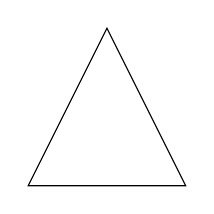
\begin{tikzpicture}
        \draw (0,0) -- (1,2) -- (2,0) -- cycle;
    \end{tikzpicture}
\end{center}

Rotaciones: 
\begin{itemize}
    \item Identidad
    \item Rotación de ángulo $\frac{2\pi}{3}$, $r_1$ $1-2-3-1$ $(1\ 2\ 3)$ $(r)$
    \item Rotación de ángulo $\frac{4\pi}{3}$, $r_2$ $1-3-2-1$ $(1\ 3\ 2)$ $(r^2)$
\end{itemize}

Simetrías: %TODO: pedir dibujo
\begin{itemize}
    \item $s_1$ $(1\ 2)$ $s$
    \item $s_2$ $(1\ 3)$ $sr = s_2$
    \item $s_3$ $(2\ 3)$ $sr^2=s_3$
\end{itemize}

\subsection{Cuadrado}

\begin{center} %TODO: terminar dibujo
    \begin{tikzpicture}
        \draw (0,0) -- (0,2) -- (2,2) -- (2,0) -- cycle;
    \end{tikzpicture}
\end{center}

Rotaciones: 
\begin{itemize}
    \item Identidad
    \item Rotación de ángulo $\frac{\pi}{2}$ $(1\ 2\ 3\ 4)$ $(r)$
    \item Rotación de ángulo $\pi$ $(1\ 3)(2\ 4)$ $(r^2)$
    \item Rotación de ángulo $\frac{3\pi}{3}$ $(1\ 4\ 3\ 2)$ $(r^3)$
\end{itemize}

Simetrías: %TODO: pedir dibujo
\begin{itemize}
    \item $s_1$: $(1\ 2)(3\ 4)$
    \item $s_2$: $(1\ 4)(2\ 3)$
    \item $s_3$: $(2\ 4)$
    \item $s_4$: $(1\ 3)$
\end{itemize}

\begin{observacion}\
    \begin{itemize}
        \item Se tiene que $sr \neq rs$
        \item Además, $sr=r^3s$ y $r=sr^3$
    \end{itemize}
\end{observacion}

La tabla de $D_4$ será:

\begin{center} % Aplicamos que rs=sr^3, sr=r^3s, s=(1 2)(3 4)
    \begin{tabular}{c|c|c|c|c|c|c|c|c|} %TODO: Terminar 
        & 1 & $r$ & $r^2$ & $r^3$ & $s$ & $sr$ & $sr^2$ & $sr^3$\\
        \hline
        1 & 1 & $r$  & $r^2$ & $r^3$ & $s$ & $sr$ & $sr^2$ & $sr^3$\\
        \hline
        $r$ & $r$ & $r^2$ & $r^3$ & 1 & $sr^3$ & $s$ & $sr$ & $sr^2$\\
        \hline
        $r^2$ & $r^2$ & $r^3$ & $1$ & $r$ & $sr^2$ & $sr^3$ & $s$ & $sr$\\
        \hline
        $r^3$ & $r^3$ & 1 & $r$ & $r^2$ & $sr$ & $sr^2$ & $sr^3$ & $s$\\
        \hline
        $s$ & $s$ & $sr$ & $sr^2$ & $sr^3$ & 1 & $r$ & $r^2$ & $r^3$\\
        \hline
        $sr$ & $sr$ & $sr^2$ & $sr^3$ & $s$ & $r^3$ & 1 & $r$ & $r^2$\\
        \hline
        $sr^2$ & $sr^2$ & $sr^3$ & $s$ & $sr$ & $r^2$ & $r^3$ & 1 & $r$\\
        \hline
        $sr^3$ & $sr^3$ & $s$ & $sr$ & $sr^2$ & $r$ & $r^2$ & $r^3$ & 1\\
        \hline
    \end{tabular}
\end{center}

\begin{align*}
    rs &=sr^{-1}\\
    rsr &=sr^{-1}r=s \\
    rsr^2 &= sr^{-1}r^2 = sr \\
    rsr^3 &= sr^{-1}r^3= sr^2\\
\end{align*}

\subsection{En general, $D_n$}

$D_n$ son las isometrías que dejan fijo un polígono regular de $n$ lados.
Tendremos $2n$ elementos:
\begin{itemize}
    \item $n$ rotaciones $\frac{2k\pi}{n} = r_k$, $k=0,\dots,n-1$.
    \item $n$ simetrías, $s_1,\dots,s_n$
\end{itemize}
Si $n$ es par tendremos $\frac{n}{2}$ diagonales y $\frac{n}{2}$ mediatrices. Si $n$ es impar tendremos $n$ radios que irán desde un vértice hasta el punto medio del lado opuesto.

\begin{notacion}
    \begin{align*}
        r &\equiv \text{rotación de ángulo }\frac{2\pi}{n}\\
        s & \equiv \text{ simetría que pasa por el origen de coordenadas y el vértice }1\ (s=s_1)
    \end{align*}
\end{notacion}

\begin{lema}\
    \begin{enumerate}
        \item $1,r,r^2,\dots,r^{n-1}$ son todos distintos y $r^n=1$ ($(O(r)=n)$)
        \item $s^2=1$, $O(s)=2$
        \item $s\neq r^i$\ \  $\forall\ 0 \leq i \leq n-1$ ($s$ fija el $1$ pero las rotaciones no).
        \item $sr^i$, $0\leq i \leq n-1$ son simetrías en los ejes de simetrías ($s_2, s_3,\dots,s_n$) y $sr^i\neq sr^j$ para $i\neq j$.
        \item $sr=r^{-1}s$ y en general $sr^i = r^{-i}s$
    \end{enumerate}
\end{lema}

\begin{ejemplo}
    En $D_2$ tenemos que $sr^9sr^6 = r^9$
\end{ejemplo}

\begin{definicion}
    Un conjunto de generadores de un grupo $G$ es un subconjunto $S\subset G$ tal que todo elemento de $G$ puede escribirse como producto finito de elementos de $S$ y sus inversos. Lo notaremos como $G=<S>$ o, en el caso de $S=\{x_1,\dots,x_n\}$ podremos escribir $G=<x_1,\dots,x_n>$ y diremos que $G$ está generado por $S$.\\

    Cualquier elemento $x\in G$ podremos escribirlo como
    \begin{align*}
        x=x_1^{\gamma_1}x_2^{\gamma_2}\dots x_n^{\gamma_n}\ \ x_i\in S,\ \ \gamma_i=\pm1
    \end{align*}
\end{definicion}

\begin{ejemplo}\
    \begin{enumerate}
        \item $G=<x>$, $S=<x>$ es un grupo cíclico. $\bb{Z}=<1>$
        \item $D_n=<r,s>$
    \end{enumerate}
\end{ejemplo}

\begin{definicion}
    Si $G=<S>$ y existe un conjunto de relaciones $R_1,R_2,\dots,R_m$ (igualdades entre elementos de $S\cup\{1\}$) tal que cualquier relación entre los elementos de $S$ puede deducirse de estas, entonces decimos que estos generadores y relaciones constituyen una \textbf{presentación de} $G$ y lo escribimos como
    \begin{align*}
        G=<S /R_1,R_2,\dots,R_m>
    \end{align*}
\end{definicion}

\begin{ejemplo}\
    \begin{enumerate}
        \item $D_n=<r,s /rs=sr^{-1}>$ (presentación abstracta de $D_n$).\\ 
        Podemos considerar $D_1=<s/s^2=1>$ y $D_2=<r,s / r^2=s^2=1, sr=rs>$ que no tienen sentido geométrico pero sí abstracto.

        \item $C_n=<x / x^n=1>=\{1,x,x^2,\dots,x^{n-1}\}$ es el grupo cíclico de orden $n$.
        \item $V^{abs} = <x,y / x^2=1,\ y^2,\ (xy)^2=1>=<1,x,y,xy>$ es el grupo de Klein abstracto
        \item $Q_2^{abs} = <x,y/x^4=1,\ y^2=x^2,\ yxy^{-1}=x^{-1}>$ es el grupo de cuaternios abstracto. %$Q_2=\{\pm 1, \pm i, \pm j, \pm k\}$ (cuaternios).
        Tenemos que $Q_2^{abs}=\{1,x,x^2,x^3,y,xy,x^2y,x^3y\}$, $O(x)=4$, $|Q_2^{abs}|=8$, $O(x^2)=2$, los demás tienen orden 4.\\

        Podemos identificar este grupo con $SL_2(\bb{C})$ de la siguiente forma:
        \begin{gather*}
            1 = 
            \begin{pmatrix}
                1 & 0\\
                0 & 1\\
            \end{pmatrix}
            \hspace{1cm}
            x = 
            \begin{pmatrix}
                i & 0\\
                0 & -i\\
            \end{pmatrix}
            \hspace{1cm}
            y = 
            \begin{pmatrix}
                0 & -1\\
                1 & 0\\
            \end{pmatrix}
            \hspace{1cm}
            x^2 = 
            \begin{pmatrix}
                -1 & 0\\
                0 & -1\\
            \end{pmatrix}\\\\
            x^3 = 
            \begin{pmatrix}
                -i & 0\\
                0 & i\\
            \end{pmatrix}
            \hspace{1cm}
            xy = 
            \begin{pmatrix}
                0 & -i\\
                -i & 0\\
            \end{pmatrix}
            \hspace{1cm}
            x^2y = 
            \begin{pmatrix}
                0 & 1\\
                -1 & 0\\
            \end{pmatrix}
            \hspace{1cm}
            x^3y = 
            \begin{pmatrix}
                0 & i\\
                i & 0\\
            \end{pmatrix}
        \end{gather*}
        y tenemos los Cuaternios $Q_2=\{\pm 1, \pm i, \pm j, \pm k\}$ y se tiene que $i^2=j^2=k^2=-1$ y además se verifica
        \begin{gather*}
            ij=k \hspace{1cm} jk=i \hspace{1cm} ki=j\\
            ji=-k \hspace{1cm} kj=-i \hspace{1cm} ik=-j
        \end{gather*}
        y podemos hacer la siguiente identificación:
        \begin{gather*}
            1 = 
            \begin{pmatrix}
                1 & 0\\
                0 & 1\\
            \end{pmatrix} \equiv 1
            \hspace{1cm}
            x = 
            \begin{pmatrix}
                i & 0\\
                0 & -i\\
            \end{pmatrix} \equiv i
            \hspace{1cm}
            y = 
            \begin{pmatrix}
                0 & -1\\
                1 & 0\\
            \end{pmatrix} \equiv j \\\\
            \hspace{1cm}
            x^2 = 
            \begin{pmatrix}
                -1 & 0\\
                0 & -1\\
            \end{pmatrix} \equiv -1
            \hspace{1cm}
            x^3 = 
            \begin{pmatrix}
                -i & 0\\
                0 & i\\
            \end{pmatrix} \equiv -i
            \hspace{1cm}
            xy = 
            \begin{pmatrix}
                0 & -i\\
                -i & 0\\
            \end{pmatrix} \equiv k\\\\
            x^2y = 
            \begin{pmatrix}
                0 & 1\\
                -1 & 0\\
            \end{pmatrix} \equiv -j
            \hspace{1cm}
            x^3y = 
            \begin{pmatrix}
                0 & i\\
                i & 0\\
            \end{pmatrix} \equiv -k
        \end{gather*}
        de esta forma hemos identificado el grupo $Q_2^{abs}$ con $Q_2$ (la presentación con el grupo descrito por sus elementos).
    \end{enumerate}
\end{ejemplo}

\section{Grupos Simétricos ($S_n$)}

Este grupo lo construiremos a partir de las permutaciones. Dado un conjunto $X$, podemos definir el conjunto de aplicaciones biyectivas 
\begin{gather*}
    S(X)=\{f:X \to X \text{ biyectivas}\}
\end{gather*}
que ya se ha trabajado como el conjunto de permutaciones. Dado $X=\{1,\dots,n\}$ finito podemos considerar el n-ésimo grupo simétrico $S(X)=S_n$ (con la composición). Se va a verificar que $|S_n|=n!$. \\

Una forma de representar los elementos $\sigma \in S_n$ es con la \textbf{representación matricial}
\begin{align*}
    \begin{pmatrix}
        1 & 2 & 3 & \dots & n\\
        \sigma(1) & \sigma(2) & \sigma(3) & \dots & \sigma(n)
    \end{pmatrix}
\end{align*}

 \begin{ejemplo}
    $S_5$ podemos describirlo matricialmente de la siguiente forma:
    \begin{align*}
        \sigma=\begin{pmatrix}
            1 & 2 & 3 & 4 & 5\\
             2 & 3 & 4 & 5 & 1
        \end{pmatrix} \leadsto (1\ 2\ 3\ 4\ 5)
        \hspace{1cm}
        \tau=\begin{pmatrix}
            1 & 2 & 3 & 4 & 5\\
            3 & 4 & 5 & 1 & 2
        \end{pmatrix} \leadsto (1\ 3)(2\ 4\ 5)\\\\
        \sigma\tau=\begin{pmatrix}
            1 & 2 & 3 & 4 & 5\\
            4 & 5 & 2 & 1 & 3
        \end{pmatrix} \leadsto (1\ 4)(2\ 5\ 3)
        \hspace{1cm}
        \tau\sigma=\begin{pmatrix}
            1 & 2 & 3 & 4 & 5\\
            4 & 1 & 5 & 2 & 3
        \end{pmatrix} \leadsto (1\ 4\ 2)(3\ 5)
    \end{align*}
    Esta segunda representación (la que aparece a continuación de la matricial) es la representación en ciclos disjuntos. No siempre tienen que variar los elementos
 \end{ejemplo}

 \begin{definicion}
    Sea $\sigma\in S_n$ tal que desplaza circularmente al conjunto $\{a_1,a_2,\dots,a_m\}\subseteq X$ y al resto de elementos los deja fijos (no se desplazan). Esto será un \textbf{ciclo de longitud} $m$.\\

    Es indiferente el primer elemento de estos ciclos de forma que
    \begin{align*}
        \sigma=(a_1,a_2,\dots,a_m) = (a_2,a_3,\dots,a_m,a_1) = \dots = (a_m, a_1, \dots, a_{m-1})
    \end{align*}
    Tendremos $\dfrac{V_m^n}{m}$ ciclos de longitud $m$.
 \end{definicion}

 \begin{ejemplo}
    En $S_5$ tendremos $\dfrac{V_5^2}{2}$ ciclos de longitud $2$ y $\dfrac{V_5^3}{3}$ ciclos de longitud $3$.
 \end{ejemplo}

 \begin{lema}\
    \begin{itemize}
        \item El orden de un ciclo de longitud $m$ es $m$.
        \item Dado $\sigma=(a_1,a_2,\dots,a_m) \leadsto \sigma^{-1}=(a_m, a_{m-1},\dots,a_2, a_1)$.
    \end{itemize} 
 \end{lema}

 \begin{definicion}
    Los 2-ciclos los llamaremos \textbf{trasposiciones}
 \end{definicion}

 \begin{definicion}
     Podemos descomponer cualquier ciclo en ciclos disjuntos de distinta longitud de la forma
     \begin{align*}
        \sigma = (a_1,a_2,\dots,a_{m_1})(a_{m_1+1}, a_{m_1+2}, \dots, a_{m_2})\dots(a_{m_k+1}, a_{m_k+2},\dots,a_{m_{k+1}})
     \end{align*}
     y lo llamaremos \textbf{descomposición en ciclos disjuntos}.\\

     De esta forma tendremos que $\sigma(a_k)=a_{k+1}$ para cualquier elemento de un ciclo que no sea el último, $\sigma(a_n)=a_{1}$ para el último elemento del ciclo y $\sigma(a_j)=a_j$ para todo elemento que no esté en el ciclo.
 \end{definicion}

 \begin{ejemplo}
    Consideramos $S_{13}$ la siguiente representación matricial:
    \begin{align*}
        \sigma = \left(
        \begin{array}{ccccccccccccc}
            1 & 2 & 3 & 4 & 5 & 6 & 7 & 8 & 9 & 10 & 11 & 12 & 13\\
            12 & 13 & 3 & 1 & 11 & 9 & 5 & 10 & 6 & 4 & 7 & 8 & 2
        \end{array}
        \right)
    \end{align*}
    Tendremos que la descomposición en ciclos disjuntos será
    \begin{align*}
        \sigma = (1\ 12\ 8\ 10\ 4)(2\ 13)(3)(5\ 11\ 7)(6\ 9)
    \end{align*}
    Tenemos que el inverso por tanto será
    \begin{align*}
        \sigma = (4\ 10\ 8\ 12\ 1)(2\ 13)(7\ 11\ 5)(6\ 9)
    \end{align*}
    Por ejemplo, tenemos que $\sigma(7)=5$
 \end{ejemplo}

 \begin{observacion}\
    \begin{itemize}
        \item Si $\sigma \in S_n$, entonces $\sigma\in S_m$ para todo $m\geq n$.
        \item En general, $S_n$ no es abeliano para $n\geq 3$
    \end{itemize}
 \end{observacion}

 \begin{ejercicio}(Ejercicio 14 de la Relación)\\
    Sean $s_1, s_2\in S_7$ dados por
    \begin{gather*}
        s_2=\begin{pmatrix}
            1 & 2 & 3 & 4 & 5 & 6 & 7\\
            5 & 7 & 6 & 2 & 1 & 4 & 3
        \end{pmatrix}
        \hspace{1cm}
        s_1=\begin{pmatrix}
            1 & 2 & 3 & 4 & 5 & 6 & 7\\
            3 & 2 & 4 & 5 & 1 & 7 & 6
        \end{pmatrix}
    \end{gather*}
    Calculamos los siguientes elementos:
    \begin{gather*}
        s_1s_2=\begin{pmatrix}
            1 & 2 & 3 & 4 & 5 & 6 & 7\\
            1 & 6 & 7 & 2 & 3 & 5 & 4
        \end{pmatrix} 
        \hspace{1cm}
        s_2s_1=\begin{pmatrix}
            1 & 2 & 3 & 4 & 5 & 6 & 7\\
            6 & 7 & 2 & 1 & 5 & 3 & 4
        \end{pmatrix}\\\\
        s_2^2=\begin{pmatrix}
            1 & 2 & 3 & 4 & 5 & 6 & 7\\
            1 & 3 & 4 & 7 & 5 & 2 & 6
        \end{pmatrix}
    \end{gather*}
    Los podemos expresar en ciclos disjuntos como
    \begin{gather*}
        s_1s_2=(2\ 6\ 5\ 3\ 7\ 4)\hspace{1cm} s_2s_1=(1\ 6\ 3\ 2\ 7\ 4)\\
        s_2^2=(2\ 3\ 4\ 7\ 6)
    \end{gather*}
 \end{ejercicio}

